%%%%%%%%%%%%%%%%%%%%%%%%%%%%%%%%%%%%%%%%%
% Short Sectioned Assignment
% LaTeX Template
% Version 1.0 (5/5/12)
%
% This template has been downloaded from:
% http://www.LaTeXTemplates.com
%
% Original author:
% Frits Wenneker (http://www.howtotex.com)
%
% License:
% CC BY-NC-SA 3.0 (http://creativecommons.org/licenses/by-nc-sa/3.0/)
%
%%%%%%%%%%%%%%%%%%%%%%%%%%%%%%%%%%%%%%%%%

%----------------------------------------------------------------------------------------
%	PACKAGES AND OTHER DOCUMENT CONFIGURATIONS
%----------------------------------------------------------------------------------------

\documentclass[paper=a4, fontsize=11pt]{scrartcl} % A4 paper and 11pt font size

\usepackage[T1]{fontenc} % Use 8-bit encoding that has 256 glyphs
\usepackage{fourier} % Use the Adobe Utopia font for the document - comment this line to return to the LaTeX default
\usepackage[english]{babel} % English language/hyphenation
\usepackage{amsmath,amsfonts,amsthm} % Math packages

\usepackage{lipsum} % Used for inserting dummy 'Lorem ipsum' text into the template

\usepackage{sectsty} % Allows customizing section commands
\allsectionsfont{\centering \normalfont\scshape} % Make all sections centered, the default font and small caps

\usepackage{fancyhdr} % Custom headers and footers

% my packages
\usepackage{commath}
\usepackage{mathtools}
\usepackage{graphicx}
\usepackage{algorithm}
\usepackage[]{algpseudocode}
\DeclarePairedDelimiter{\ceil}{\lceil}{\rceil}
\usepackage{tikz}
\usepackage{pgfplots}
\pgfplotsset{compat=newest}
\usetikzlibrary{shapes.geometric,arrows,fit,matrix,positioning}
\tikzset
{
    treenode/.style = {white, circle, draw=black, fill=black, align=center, minimum size=1cm},
    nvnode/.style = {circle, draw=black, align=center, minimum size=1cm},
    optnode/.style = {circle, draw=red, red, align=center, minimum size=1cm},
    subtree/.style  = {isosceles triangle, draw=black, align=center, minimum height=0.5cm, minimum width=1cm, shape border rotate=90, anchor=north}
}

\pagestyle{fancyplain} % Makes all pages in the document conform to the custom headers and footers
\fancyhead{} % No page header - if you want one, create it in the same way as the footers below
\fancyfoot[L]{} % Empty left footer
\fancyfoot[C]{} % Empty center footer
\fancyfoot[R]{\thepage} % Page numbering for right footer
\renewcommand{\headrulewidth}{0pt} % Remove header underlines
\renewcommand{\footrulewidth}{0pt} % Remove footer underlines
\setlength{\headheight}{13.6pt} % Customize the height of the header

\numberwithin{equation}{section} % Number equations within sections (i.e. 1.1, 1.2, 2.1, 2.2 instead of 1, 2, 3, 4)
\numberwithin{figure}{section} % Number figures within sections (i.e. 1.1, 1.2, 2.1, 2.2 instead of 1, 2, 3, 4)
\numberwithin{table}{section} % Number tables within sections (i.e. 1.1, 1.2, 2.1, 2.2 instead of 1, 2, 3, 4)

\setlength\parindent{0pt} % Removes all indentation from paragraphs - comment this line for an assignment with lots of text

% new commands
\newcommand{\filename}[1]{\textbf{\textit{#1}}}
\newcommand{\funcname}[1]{\textbf{#1}}
\newcommand{\inv}{^{\raisebox{.2ex}{$\scriptscriptstyle-1$}}}
\renewcommand{\vec}[1]{\mathbf{#1}}

\makeatletter
\renewcommand*\env@matrix[1][*\c@MaxMatrixCols c]{%
  \hskip -\arraycolsep
  \let\@ifnextchar\new@ifnextchar
  \array{#1}}
\makeatother

\makeatletter
\def\BState{\State\hskip-\ALG@thistlm}
\makeatother

\DeclareMathOperator*{\argmin}{arg\,min} % Jan Hlavacek

%----------------------------------------------------------------------------------------
%	TITLE SECTION
%----------------------------------------------------------------------------------------

\newcommand{\horrule}[1]{\rule{\linewidth}{#1}} % Create horizontal rule command with 1 argument of height

\title{	
\normalfont \normalsize 
\textsc{Mathematical foundations of computer graphics and vision} \\ [25pt] % Your university, school and/or department name(s)
\horrule{0.5pt} \\[0.4cm] % Thin top horizontal rule
\huge Exercise 2. Global Optimization \\ % The assignment title
\horrule{2pt} \\[0.5cm] % Thick bottom horizontal rule
}

\author{Dongho Kang \\ \small 16-948-598} % Your name

\date{\normalsize March 19, 2017} % Today's date or a custom date

\begin{document}

\maketitle % Print the title

%----------------------------------------------------------------------------------------
%	README
%----------------------------------------------------------------------------------------

MATLAB R2016b version was used for coding and testing:

\begin{center}
MathWorks, MATLAB R2016b (9.1.0.441655) \\
64-bit (maci64) 
\end{center}

The \filename{code} directory contains followings:

\begin{itemize}
	\item \filename{main.m} \quad Script .m file for exercise.
	\item \filename{functions dir} \quad Function .m files 
		\begin{itemize}
			\item \funcname{SolveWithLP} \quad Function .m file for solving a problem with the LP and simple testing.
			\item \funcname{SplitProblem} \quad Function .m file for split a parent problem into two children problems.
			\item \funcname{FindBestCandidate} \quad Function .m file for finding the best candidate between two children node.
			\item \funcname{PushToStack} \quad Function .m file for stack push operation.
			\item \funcname{PopFromStack} \quad Function .m file for stack pop operation.
			\item \funcname{NewProblem} \quad Function .m file for creating new problem (instance of struct).    
			\item \funcname{FindInliers} \quad Function .m file for finding inliers with a input model.    
			\item and other sub-functions: \funcname{VisualizeMatch}, \funcname{SaveOptHistory}, \funcname{ComputeInlierLb}
		\end{itemize}
	\item \filename{data dir} \quad data and image files provided.
\end{itemize}

For running exercise, adjust threshold parameter (default of 3 pixel) and run the \filename{main.m} on the MATLAB environment. More details are stated in the \textit{Running} section.

%----------------------------------------------------------------------------------------
%	PROBLEM 1
%----------------------------------------------------------------------------------------

\section{exercise : Branch and bound for consensus set maximization}

%----------------------------------------------------------------------------------------
%	DESCRIPTION
%----------------------------------------------------------------------------------------
\subsection{Description}

In this exercise, branch and bound algorithm based on depth-first search(DFS) was implemented. The implementation steps are as follows: 

\begin{itemize}
\item derivation of the problem formulation in the canonical form of the linear programming
\item branch and bound algorithm implementation
\item logging and plotting the result of branch and bound algorithm
\end{itemize}  

%----------------------------------------------------------------------------------------
\subsubsection{Linear Programming Formulation}

Let the set $S$ of the input data be partitioned into an inlier-set $S_{I} \subseteq S$ and an outlier-set $S_{O} = S \setminus S_{I}$. Note that  

\begin{itemize}
\item the model $\Theta = (T_{x}, T_{y})$ where $T_{x}$ and $T_{y}$ represent the translation along the $x$ and $y$ axis.
\item the i-th input correspondence is $(p_{i}, p_{i}')$ where $p_{i}$ and $p_{i}'$ represent the points in the left and right images: $p_{i} = (x_{i}, y_{i})$ and $p_{i} = (x_{i}', y_{i}')$. There are $n$ input correspondences.
\end{itemize}

then the consensus set maximization problem can be formulated as follows: 

\begin{equation}
\begin{split}
\max_{\Theta, S_{I}} &\quad card(S_{I}) \\
s.t. 	&\quad \abs{x_{i} + T_{x} - x_{i}'} \leq \delta, \forall i \in S_{I} \subseteq S \\
	&\quad \abs{y_{i} + T_{y} - y_{i}'} \leq \delta, \forall i \in S_{I} \subseteq S
\end{split}
\end{equation}

To solve the problem by linear programming, alternative formulation using $z_{i}$ and the relaxation can be applied to (1.1):

\begin{align}
\max_{\Theta, \vec{z}} &\quad \sum_{i=1}^{N} z_{i} \\
s.t. 	&\quad z_{i}\abs{x_{i} + T_{x} - x_{i}'} \leq z_{i} \delta, \forall i \in S_{I} \subseteq S \\
	and &\quad z_{i}\abs{y_{i} + T_{y} - y_{i}'} \leq z_{i} \delta, \forall i \in S_{I} \subseteq S \\
	and &\quad z_{i} \in [0, 1], \quad \forall i = 1 \dots N \\
	and &\quad \underbar{$T_{x}$} \leq T_{x} \leq \overline{T_{x}},
	\quad \underbar{$T_{y}$} \leq T_{y} \leq \overline{T_{y}}, \quad \forall i = 1 \dots N 
\end{align}

(1.3) and (1.4) can be expressed into:

\begin{equation}
\begin{split}
\quad - z_{i} \delta \leq z_{i} (x_{i} + T_{x} - x_{i}') \leq z_{i} \delta \\
\quad - z_{i} \delta \leq z_{i} (y_{i} + T_{y} - y_{i}') \leq z_{i} \delta 
\end{split}
\end{equation}

Now, introducing the auxiliary variables $w_{ix} = z_{i}T_{x}$ and $w_{iy} = z_{i}T_{y}$ to avoid the bilinear terms, (1.6) can be relaxed by concave and convex envelopes:

\begin{equation}
\begin{split}
w_{ix} = z_{i} T_{x} &\geq \max(\underbar{$z_{i}$} T_{x} + \underbar{$T_{x}$}z_{i} - \underbar{$z_{i}$}\underbar{$T_{x}$},
 	\overline{z_{i}} T_{x} + \overline{T_{x}}z_{i} - \overline{z_{i}} \overline{T_{x}}) \\
w_{ix} = z_{i} T_{x} &\leq \min(\overline{z_{i}}T_{x} + \underbar{$T_{x}$}z_{i} - \overline{z_{i}} \underbar{$T_{x}$}, 
	 \underbar{$z_{i}$} T_{x} + \overline{T_{x}}z_{i} - \underbar{$z_{i}$} \overline{T_{x}})
\end{split}
\end{equation}

$\max$ and $\min$ is not a linear function, thus changed (1.8) into the following forms:

\begin{equation}
\begin{split}
w_{ix} &\geq \underbar{$z_{i}$} T_{x} + \underbar{$T_{x}$}z_{i} - \underbar{$z_{i}$}\underbar{$T_{x}$} \\
w_{ix} &\geq \overline{z_{i}} T_{x} + \overline{T_{x}}z_{i} - \overline{z_{i}} \overline{T_{x}} \\
w_{ix} &\leq \overline{z_{i}}T_{x} + \underbar{$T_{x}$}z_{i} - \overline{z_{i}} \underbar{$T_{x}$} \\
w_{ix} &\leq \underbar{$z_{i}$} T_{x} + \overline{T_{x}}z_{i} - \underbar{$z_{i}$} \overline{T_{x}}
\end{split}
\end{equation}

changed (1.8) into linear programming constraint form:

\begin{equation}
\begin{split}
\underbar{$z_{i}$} T_{x} + \underbar{$T_{x}$}z_{i} - w_{ix} &\leq \underbar{$z_{i}$}\underbar{$T_{x}$} \\
\overline{z_{i}} T_{x} + \overline{T_{x}}z_{i} - w_{ix} &\leq \overline{z_{i}} \overline{T_{x}} \\
- \overline{z_{i}}T_{x} - \underbar{$T_{x}$}z_{i} + w_{ix} &\leq  -\overline{z_{i}} \underbar{$T_{x}$} \\
- \underbar{$z_{i}$} T_{x} - \overline{T_{x}}z_{i} + w_{ix} &\leq -\underbar{$z_{i}$} \overline{T_{x}}
\end{split}
\end{equation}

likewise, $w_iy$: 

\begin{equation}
\begin{split}
\underbar{$z_{i}$} T_{y} + \underbar{$T_{y}$}z_{i} - w_{iy} &\leq \underbar{$z_{i}$}\underbar{$T_{y}$} \\
\overline{z_{i}} T_{y} + \overline{T_{y}}z_{i} - w_{iy} &\leq \overline{z_{i}} \overline{T_{y}} \\
- \overline{z_{i}}T_{y} - \underbar{$T_{y}$}z_{i} + w_{iy} &\leq  -\overline{z_{i}} \underbar{$T_{y}$} \\
- \underbar{$z_{i}$} T_{y} - \overline{T_{y}}z_{i} + w_{iy} &\leq - \underbar{$z_{i}$} \overline{T_{y}}
\end{split}
\end{equation}

and finally, as $w_{ix} = z_{i}T_{x}$ and $w_{iy} = z_{i}T_{y}$, (1.7) can be expressed into:

\begin{equation}
\begin{split}
\quad z_{i} x_{i} + w_{ix} - z_{i} x_{i}' - z_{i} \delta \leq  0\\
\quad - z_{i} x_{i} - w_{ix} + z_{i} x_{i}' - z_{i} \delta \leq  0\\
\quad z_{i} y_{i} + w_{iy} - z_{i} y_{i}' - z_{i} \delta \leq  0\\
\quad - z_{i} y_{i} - w_{iy} + z_{i} y_{i}' - z_{i} \delta \leq  0\\
\end{split}
\end{equation}

Now, as MATLAB function \funcname{linprog} solve following problem,

\begin{equation}
\begin{split}
\min_{x} c^{T}\vec{x} \\
s.t. A\vec{x} \leq b \\
l_{b} \leq \vec{x} \leq u_{b} 
\end{split}
\end{equation}

set the unknown vector, coefficient vector, and $l_{b}, u_{b}$ vectors for linear programming to

\begin{equation}
\begin{split}
\vec{x} &= (T_{x}, T_{y}, z_{1}, \dots, z_{n}, w_{1x}, \dots, w_{nx}, w_{1y}, \dots, w_{ny})^{T} \\
l_{b} &= (\underbar{$T_{x}$}, \underbar{$T_{y}$}, \underbar{$z_{1}$}, \dots, \underbar{$z_{n}$}, -\infty, \dots, -\infty)^{T} \\
u_{b} &= (\overline{T_{x}}, \overline{T_{y}}, \overline{z_{1}}, \dots, \overline{z_{n}}, \infty, \dots, \infty)^{T} \\
c &= (0, 0, -1, \dots, -1, 0, \dots, 0)^{T}
\end{split}
\end{equation}

Note that coefficient vector c is $c^{T} \vec{x} = - z_{1} - z_{2} - \dots - z_{n}$. This is for making the maximizing problem into the minimizing problem. Besides, $-\infty \leq w_{ix} \leq \infty$ and $-\infty \leq w_{iy} \leq \infty$, because there is no either lower nor upper bound for $w_{ix}$ and $w_{iy}$. \\ Lastly, (1.9), (1.10) and (1.11) was changed into the form of (1.12). Thus, matrix $A$ and vector $b$ are as follows:

\begin{equation*}
A_{i} = 
\begin{bmatrix}[c c | c c c c c | c c c c c | c c c c c ]
	0 & 0 &	0 & \dots & (x_{i} - x_{i}' - \delta) & \dots & 0		& 0 & \dots & 1 & \dots & 0 	& 0 & \dots & 0 & \dots & 0 \\
	0 & 0 &	0 & \dots & (-x_{i} + x_{i}' - \delta) & \dots & 0		& 0 & \dots & -1 & \dots & 0 	& 0 & \dots & 0 & \dots & 0 \\
	0 & 0 &	0 & \dots & (y_{i} - y_{i}' - \delta) & \dots & 0		& 0 & \dots & 0 & \dots & 0 	& 0 & \dots & 1 & \dots & 0 \\
	0 & 0 &	0 & \dots & (-y_{i} + y_{i}' - \delta) & \dots & 0		& 0 & \dots & 0 & \dots & 0 	& 0 & \dots & -1 & \dots & 0 \\
	\underbar{$z_{i}$} & 0 &	0 & \dots & \underbar{$T_{x}$} & \dots & 0	& 0 & \dots & -1 & \dots & 0 	& 0 & \dots & 0 & \dots & 0 \\
	\overline{z_{i}} & 0 &		0 & \dots & \overline{T_{x}} & \dots & 0		& 0 & \dots & -1 & \dots & 0 	& 0 & \dots & 0 & \dots & 0 \\
	-\overline{z_{i}} & 0 &	0 & \dots & -\underbar{$T_{x}$} & \dots & 0	& 0 & \dots & 1 & \dots & 0 	& 0 & \dots & 0 & \dots & 0 \\
	-\underbar{$z_{i}$} & 0 &	0 & \dots & -\overline{T_{x}} & \dots & 0		& 0 & \dots & 1 & \dots & 0 	& 0 & \dots & 0 & \dots & 0 \\
	0 & \underbar{$z_{i}$} & 	0 & \dots & \underbar{$T_{y}$} & \dots & 0	& 0 & \dots & 0 & \dots & 0 	& 0 & \dots & -1 & \dots & 0 \\
	0 & \overline{z_{i}} & 	0 & \dots & \overline{T_{y}} & \dots & 0		& 0 & \dots & 0 & \dots & 0 	& 0 & \dots & -1 & \dots & 0 \\
	0 & -\overline{z_{i}} & 	0 & \dots & -\underbar{$T_{y}$} & \dots & 0	& 0 & \dots & 0 & \dots & 0 	& 0 & \dots & 1 & \dots & 0 \\
	0 & -\underbar{$z_{i}$} & 	0 & \dots & -\overline{T_{y}} & \dots & 0		& 0 & \dots & 0 & \dots & 0 	& 0 & \dots & 1 & \dots & 0 
\end{bmatrix} 
\end{equation*} 

\begin{align*}
b_{i} &= 
\begin{bmatrix}
	0 \\ 0 \\ 0 \\ 0 \\ 
        \underbar{$z_{i}$}\underbar{$T_{x}$} \\
        \overline{z_{i}} \overline{T_{x}} \\
        -\overline{z_{i}} \underbar{$T_{x}$} \\
        -\underbar{$z_{i}$} \overline{T_{x}} \\
        \underbar{$z_{i}$}\underbar{$T_{y}$} \\
        \overline{z_{i}} \overline{T_{y}} \\
        -\overline{z_{i}} \underbar{$T_{y}$} \\
        -\underbar{$z_{i}$} \overline{T_{y}}
\end{bmatrix} &
A &=  
\left[ \begin{array}{c}
	A_{1} \\
	\hline 
	A_{2} \\
	\hline
	\vdots \\
	\hline
	A_{n} 
\end{array} \right] &
b &= 
\left[ \begin{array}{c}
	b_{1} \\
	\hline 
	b_{2} \\
	\hline
	\vdots \\
	\hline
	b_{n} 
\end{array} \right]
\end{align*} \\

Note that $\underbar{$z_{i}$} = 0$ and $\overline{z_{i}} = 1$. For avoiding a loop, $A$ and $b$ was reformed in the MATLAB implementation.


%----------------------------------------------------------------------------------------
\subsubsection{Branch and bound}

Implemented branch and bound algorithm for finding optimal solution of the consensus set maximization problem. The depth-first search based on stack data structure was used. The stack has two operation \funcname{PopFromStack} and \funcname{PushToStack}. \\

The pseudo-code of the implementation is as follows: 

\begin{algorithm}
\caption{Branch and bound}\label{euclid}
\begin{algorithmic}[1]
\State \textit{P0} $\gets$ whole problem space
\State init. $\textit{opt}$ $\gets$ variable for optimal solution (bound of inliers)
\State init. $\textit{stack}$ 
\State \textit{push(stack, P0)}
\State 
\While {\textit{stack} is not empty}
	\State \textit{Parent} = \textit{pop(stack)}
	\If {\textit{Parent.ObjUpperBound} < \textit{opt.LowerBound} } 
		\State \textbf{continue;} $\gets$ bad bound. does not contain optimum for sure
	\EndIf
	\State
	\If {$\textit{Parent.ObjLowerBound} \geq \textit{opt.LowerBound}$}
        		\State \textit{opt} = (\textit{Parent.ObjUpperBound, Parent.ObjLowerBound})
        \EndIf
        	\State
	\If {$\textit{Parent.ObjUpperBound} - \textit{Parent.ObjLowerBound} < 1$}
        		\State \textbf{continue;} $\gets$ \textit{Parent} is a leaf node thus do not split
        \EndIf
        \State
        \State (\textit{LeftChild, RightChild}) = \textit{split(Parent)}
        \State \textit{solveLP(LeftChild, RightChild)} $\gets$ solve both problems by LP and test
	\State
	\State \textit{(BetterChild, WorseChild) = findbetter(LeftChild, RightChild)}
	\State \textit{push(stack, WorseChild)}	
	\State \textit{push(stack, BetterChild)} $\gets$ \textit{BetterChild} should be on the top of stack
\EndWhile
\State
\State \textit{opt} $\gets$ now optimal solution  
\end{algorithmic}
\end{algorithm}

\pagebreak

The several criteria/strategies of implementation were defined as follows

\begin{enumerate}
\item push the original problem $P0$ to the problem stack.
\item start iteration. The iteration of branch and bound terminates when the problem stack is empty
\item bad bound check criteria: 
	\begin{itemize}
	\item $m^*$ is the highest lower bound of the number of inliers obtained so far.
	\item if the upper cardinality bound of a problem $< m^*$ then there's no optimum for sure.
	\item pop the problem from the stack without splitting.
	\end{itemize}
\item optimal solution update criteria :
	\begin{itemize}
	\item if the lower cardinality bound of a problem $lb$ is $lb \geq$ the lower cardinality bound of the optimal solution found so far, then update the optimal solution as $lb$.  
	\end{itemize}
\item convergence criteria: if the lower and upper cardinality bound are nearer than 1, stop split. 
	\begin{itemize}
	\item iteration can be terminated because the cardinality bound converged to optimum. 
	\item but here, to check whether obtained optimum is indeed global optimum, do not terminate iteration but check remaining problems by continuing depth-first search. 
	\end{itemize}
\item split the problem space and branching: splitting in half along the longest dimension. 
\item solve children problems and obtain the cardinality bound by the LP and simple test
	\begin{itemize}
	\item compute the upper bound of the number of inliers: the LP with the formulation of (1.1.1) was exploited.
	\item compute the lower bound of the number of inliers: simple test with the model $\Theta$ obtained by LP. Details are stated below.
	\end{itemize}
\item after solving children problems, push \textit{worse} child problem to the stack first, and then push \textit{better} child:
	\begin{itemize}
	\item \textit{better} child is a problem with a larger lower cardinality bound. If two children have the same lower cardinality bound, then choose one with a larger upper cardinality bound.
	\item as pushing two children, top of the stack is the \textit{better} child now. Thus the \textit{better} child will be popped in the next iteration step. 
	\item this strategy is for exploring \textit{better} problem first for reducing running time. 
	\end{itemize}
\item iteration terminates with the global optimal cardinality bound. 
\end{enumerate}

\paragraph{Solving a problem} The problem solving step is getting upper bound and lower bound of the number of inliers. Given a certain problem, solves the problem with the LP defined in (1.1.1). Then, the optimal solution of the relaxed problem $(T_{x}^*, T_{y}^*)$ and the objective cost $c^{T}\vec{x}^*$ are obtained from:

\begin{align}
\vec{x}^* &= (T_{x}^*, T_{y}^*, z_{1}^*, \dots, z_{n}^*, w_{1x}^*, \dots, w_{nx}^*, w_{1y}^*, \dots, w_{ny}^*)^{T} \\
c^{T} \vec{x}^* &= - z_{1}^* - z_{2}^* - \dots - z_{n}^*
\end{align}

The (-)objective cost, $-c^{T}\vec{x}^*$ can be set as the upper bound of inliers since the the number of inliers of that problem space never exceeds  $-c^{T}\vec{x}^*$. \\

Besides, the lower bound of inliers can be obtained by simple test with $(T_{x}^*, T_{y}^*)$ and is set as the $card(S_{I})$ as follows:

\begin{equation}
\begin{split}
card(&S_{I})  \\
s.t. 	&\quad \abs{x_{i} + T_{x}^* - x_{i}'} \leq \delta, \forall i \in S_{I} \subseteq S \\
	&\quad \abs{y_{i} + T_{y}^* - y_{i}'} \leq \delta, \forall i \in S_{I} \subseteq S
\end{split}
\end{equation}

This was implemented as the function \funcname{SolveWithLP}.

%----------------------------------------------------------------------------------------
%	RUNNING
%----------------------------------------------------------------------------------------
\subsection{Running}

Run the script \filename{main.m} after setting the parameters. 

\begin{itemize}
\item \textit{threshold} : threshold for inliers. Default is 3 (px).
\item \textit{padding} : the width of black padding between left and right image for figure(1). Default is 10 (px).
\end{itemize}

%----------------------------------------------------------------------------------------
%	RESULT
%----------------------------------------------------------------------------------------
\subsection{Result}

The optimal solution $(T_{x}^*, T_{y}^*)$ found by branch and bound for the given problem is as follows:

\begin{table}[h]
\captionof{table}{The global optimal solution obtained by branch and bound} \label{tab:title} 
\centering
\begin{tabular}{| c | c | c | }
\hline 
$T_{x}^*$		&	$T_{y}^*$		&	cardinality bound \\
\hline  
-232.00		&	-156.81		&	(15, 15.449) \\
\hline
\end{tabular}
\end{table}

Inlier indices are $(3, 8, 9, 15, 16, 20, 26, 31, 32, 34, 35, 40, 42, 45, 51)$. The identified inliers and plot of cardinality bounds are as follows. The red lines indicate outliers and the green lines indicate inliers: 

\begin{figure}[h]
\caption{The identified inlier and outlier correspondences\label{fig:simple}}
\noindent\makebox[\textwidth]{
  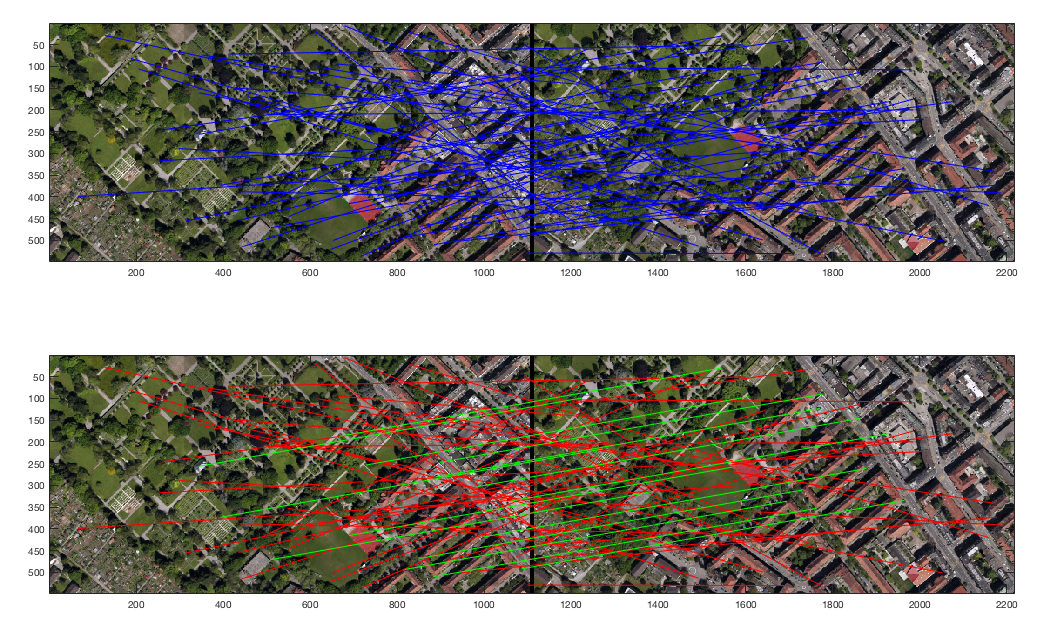
\includegraphics[width=1.0\textwidth]{inlier}
}
\end{figure} 

\begin{figure}[H]
\caption{The convergence of the cardinality bounds\label{fig:simple}}
\noindent\makebox[\textwidth]{
  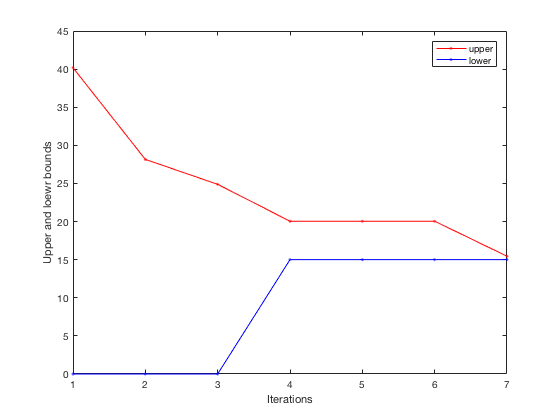
\includegraphics[width=1.0\textwidth]{cardinality_bound}
}
\end{figure} 

\pagebreak

The branch and bound iteration can be described as the following binary tree illustration:

\begin{figure}[H]
\centering
\caption{An illustration of DFS tree: one step before exploring $P11$ \label{fig:simple}}
{
    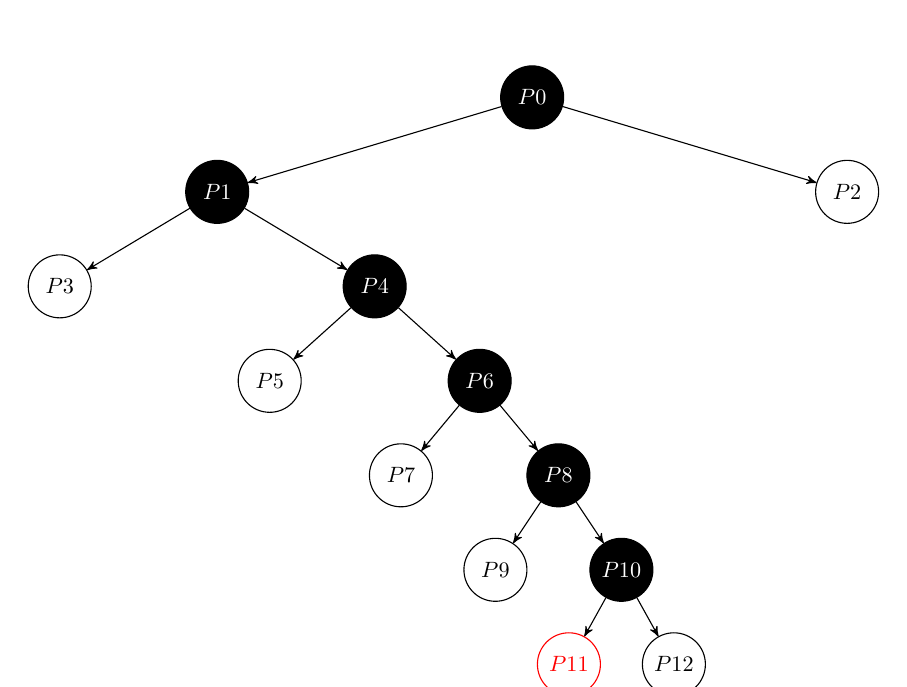
\begin{tikzpicture}[->,>=stealth', level/.style={sibling distance = 10cm/#1, level distance = 1.5cm}, scale=0.8,transform shape]
    \node [treenode] {$P0$} % (0, 40.17)
    child
    {
        node [treenode] {$P1$} %\\ (0, 28.15)} 
        child
        {
            node [nvnode] {$P3$} % \\ (0, 5.05)} 
        }
        child
        {
            node [treenode] {$P4$} % \\ (0, 24.88)}
            child 
            {
	    	node [nvnode] {$P5$} % \\ (0, 5.56)}
            }
            child 
            {
	    	node [treenode] {$P6$} % \\ (15, 20.04)}	        
		child 
            	{
	    		node [nvnode] {$P7$} % \\ (0, 2.88)}	        
            	}
		child 
            	{
	    		node [treenode] {$P8$} % \\ (0, 16.46)}	        
			child 
            		{
	    		node [nvnode] {$P9$} % \\ (0, 1.53)}	        
            		}
			child 
            		{
	        	    		node [treenode] {$P10$} %\\ (0, 15.89)}	        
        				child 
                    		{
        	    				node [optnode] {$P11$}  %\\ (15, 15.44)}	        
                    		}
				child 
                    		{
        	    				node [nvnode] {$P12$} %\\ (0, 1.37)}	        
                    		}
            		}
            	}
            }
        }
    }
    child
    {
    	node [nvnode] {$P2$} % \\ (0, 11.52)}
    }
;
% ------------------------------------------------ put the text into subtree nodes
\end{tikzpicture}
}
	\caption{An illustration of DFS stack: one step before popping $P11$ \label{fig:simple}}
	\centering
        \begin{tabular}{ | c c c c c c c }
        \hline
        P2 & P3 & P5 & P7 & P9 & P12 & P11 \\ 
        \hline
        \end{tabular} 
        
        	\caption{Problems \label{tab:title}}
	\centering
        \begin{tabular}{ | c | c | c | c | c | c |}
        \hline
         	& $\Theta_{Lb}$ 	& $\Theta_{Ub}$ 	& $\Theta_{Opt}$ 	& ObjLb & ObjUb \\ 
        \hline
        P0 & (-1104, -549)		& (1104, 549)		& (-140.94, -106.08)	& 0 & 40.17\\ 
        \hline
        P1 & (-1104, -549)		& (0, 549)			& (-336.28, -74.21)	& 0 & 28.15 \\ 
        \hline
        P2 & (0, -549) 		& (1104, 549)		& (432.47, 25.20)	& 0 & 11.52\\
        \hline
        P3  & (-1104, -549)	& (-552, 549) 		& (-665.11, -66.06)	& 0 & 5.05\\
        \hline
        P4  & (-552, -549)		& (0, 549)			& (-238.00, -154.00)	& 0 & 24.88\\
        \hline
        P5   & (-552, 0) 		& (0,549)			& (-239.45, 198.5954)	& 0 & 5.56\\ 
        \hline
        P6   & (-552, -549) 	& (-552, -549)		& (0, 0) 			& 15 & 20.04\\ 
        \hline
        P7   & (-552, -549) 	& (-276, 0) 		& (-436.00, -259.00) & 0 & 2.88\\ 
        \hline
        P8   & (-276, -549) 	& (0, 0) 			& (-232.00, -158.18)	& 0 & 16.46\\ 
        \hline
        P9   & (-276, -549) 	& (0, -275)		& (-154.00, -401.97)	& 0 & 1.53\\ 
        \hline
        P10 & (-276, -274)		& (0, 0)			& (-232.00, -156.94)	& 0 & 15.89\\
        \hline
        P11 & (-276, -274)		& (-138, 0)		& (-232.00, -156.81)	& 15 & 15.44\\
        \hline 
        P12 & (-138, -274)		& (0, 0)			& (-38.00, -99.03)	& 0 & 1.37\\
        \hline
        \end{tabular}
\end{figure}

As popping $P11$ from the stack, optimal solution is obtained but, since $P2, P3, P5, P7, P8, P12$ are still in the stack, algorithm does not terminate. However, These problems have \textit{bad bound} i.e. have smaller ObjUb (upper bound of the card.) than $P11$'s ObjLb (lower bound of the cardinality), and cannot be a optimal for sure, thus are popped without splitting and the algorithm terminates.

%----------------------------------------------------------------------------------------
%	DISCUSSION
%----------------------------------------------------------------------------------------
\subsection{Discussion}

Some comments for the bound of cardinality:

\begin{itemize}
\item The lower bound of cardinality for optimal solution monotonically increases. 
\item The upper bound of cardinality for optimal solution not necessarily monotonically decreases.
	\begin{itemize}
	\item if the first convergence (local optimal solution) is not the global optimal solution, then the upper bound of cardinality can be increased as continuing depth-first search.
	\end{itemize}
\item The global optimal solution is obtained by branch and bound algorithm. 
\end{itemize}

\end{document}